\documentclass[aspectratio=169]{beamer}

\mode<presentation> {
	\usetheme{metropolis} 
}

\usepackage{pgfpages}

\setbeamertemplate{footline}[frame number]
\addtocounter{framenumber}{-1}

\usepackage[utf8]{inputenc}
\usepackage[czech]{babel}
\usepackage{graphicx}
\usepackage{listings}
\usepackage{fontawesome}

\title[Open Source Development Course]{Open Source Development Course\\ \small Continuous integration and deployment (CI/CD)}
\author{Vojtěch Trefný\\ \small \texttt{vtrefny@redhat.com}\\}
\date{31.~3.~2021}
 \institute{\faTwitter\, \href{https://twitter.com/vojtechtrefny}{twitter.com/vojtechtrefny} \\ \faGithub\, \href{https://github.com/vojtechtrefny}{github.com/vojtechtrefny} \\ \faGitlab\ \href{https://gitlab.com/vtrefny}{gitlab.com/vtrefny}}

\begin{document}

{\setbeamertemplate{footline}{} 
\begin{frame}
\titlepage
\end{frame}
}

\newcommand*\openquote{\makebox(25,-22){\scalebox{5}{``}}}
\newcommand*\closequote{\makebox(25,-22){\scalebox{5}{''}}}

%%%%%%%%%%%%%%%%%%%%%%%%%%%%%%%%%%%%%%%%%%%%%%%%%%%%%%%%%%%%%%%%%%

\section{Pipeline}

\begin{frame}
	\frametitle{CI/CD Pipeline}

	\begin{block}{}
		\begin{itemize}
			\item Steps that need to be performed to test and deliver a new version of the software.
			\item Defines what needs to be done: when, how and in what order.
			\item Steps can vary for every project.
			\item Multiple pipelines or steps can run in parallel.
		\end{itemize}
	\end{block}
	
	\begin{figure}[ht!]
	\begin{center}
  	  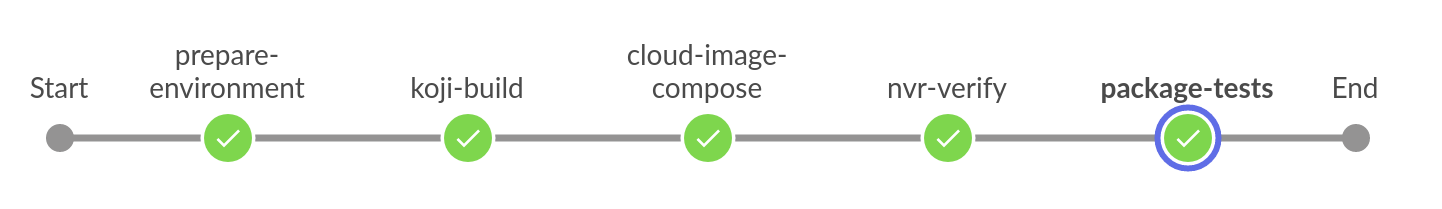
\includegraphics[width=11cm]{img/fedora-pipeline.png}
	\end{center}
	\end{figure}
\end{frame}

\begin{frame}
	\frametitle{CI/CD Pipeline}
	
\begin{columns}
\begin{column}{0.5\textwidth}
   	\begin{block}{\color{orange}{1. Testing environment}}
   		\vspace{1mm}
Preparation of the environment to run the tests: deploying containers, starting VMs...
	\end{block}
	\begin{block}{\color{orange}{2. Static Analysis}}
   		\vspace{1mm}
Finding defects by analyzing the code without running it.
     \end{block}
         \begin{block}{\color{orange}{3. Code style}}
   		\vspace{1mm}
Checking for violations of the language or project style guides.
     \end{block}
     
\end{column}
\begin{column}{0.5\textwidth}
\begin{block}{\color{orange}{4. Build}}
   		\vspace{1mm}
Building the project from source.\\~
     \end{block}
      \begin{block}{\color{orange}{5. Tests}}
   		\vspace{1mm}
Running project test suite or test suites.\\~
     \end{block}
      \begin{block}{\color{orange}{6. Packaging and Deployment}}
   		\vspace{1mm}
Building source archives, packages or container images.
     \end{block}
\end{column}
\end{columns}
\end{frame}

\section{Testing Environment}

\begin{frame}
	\frametitle{Testing Environment}

\begin{columns}
\begin{column}{0.5\textwidth}
	\begin{figure}[ht!]
	\begin{center}
  	  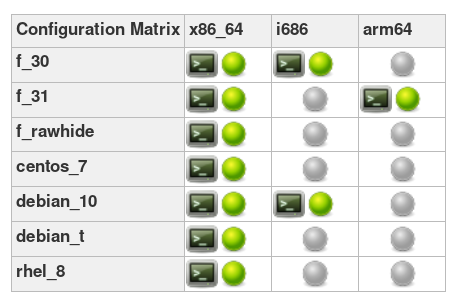
\includegraphics[width=\textwidth]{img/ci-matrix.png}
	\end{center}
	\end{figure}
\end{column}
\begin{column}{0.5\textwidth}
\begin{block}{\color{orange}{1. Preparation of VMs/containers to run the tests}}
   		\vspace{1mm}
We might want to run tests in different environments on multiple different distributions or architectures.
     \end{block}
      \begin{block}{\color{orange}{2. Installation of the test dependencies}}
   		\vspace{1mm}
Test dependencies are usually not covered by the project dependencies.
     \end{block}
      \begin{block}{\color{orange}{3. Getting the code}}
   		\vspace{1mm}
Clone the PR or get the latest code from the master branch.
     \end{block}
\end{column}
\end{columns}
\end{frame}

\section{Static Analysis}

\begin{frame}
	\frametitle{Static Analysis}

	\begin{block}{}
		\begin{itemize}
			\item Tools that can identify potential bugs by analyzing the code without running it.
			\item Can detect problems not covered by the test suite -- corner cases, error paths etc.
				\begin{itemize}
					\item Coverity (C/C++, Java, Python, Go…)\footnotemark
					\item Cppcheck (C/C++)\footnotemark
					\item Pylint (Python)\footnotemark
					\item RuboCop (Ruby)\footnotemark
				\end{itemize}
		\end{itemize}
	\end{block}

\footnotetext[1]{\tiny\url{https://scan.coverity.com}}
\footnotetext[2]{\tiny\url{http://cppcheck.sourceforge.net/}}
\footnotetext[3]{\tiny\url{https://www.pylint.org}}
\footnotetext[4]{\tiny\url{https://docs.rubocop.org}}

\end{frame}

\begin{frame}[fragile]
	\frametitle{Coverity}
\begin{lstlisting}[frame=none, basicstyle=\ttfamily\small, escapechar=$, columns=fullflexible, keepspaces=true]
$\color{red}{Error: USE\_AFTER\_FREE (CWE-825):}$
libblockdev-2.13/src/plugins/lvm-dbus.c:1163: freed_arg: "g_free" 
frees "output".
libblockdev-2.13/src/plugins/lvm-dbus.c:1165: pass_freed_arg: Passing freed 
pointer "output" as an argument to "g_set_error".
$\color{blue}{\#}$ 1163|       g_free (output);
$\color{blue}{\#}$ 1164|       if (ret == 0) {
$\color{blue}{\#}$ 1165|->         g_set_error (error, BD_LVM_ERROR, BD_LVM_ERROR_PARSE,
$\color{blue}{\#}$ 1166|                        "Failed to parse number from output: '%s'",
$\color{blue}{\#}$ 1167|                        output);
\end{lstlisting}

\end{frame}

\begin{frame}
	\frametitle{LGTM}

\begin{figure}[ht!]
	\begin{center}
  	  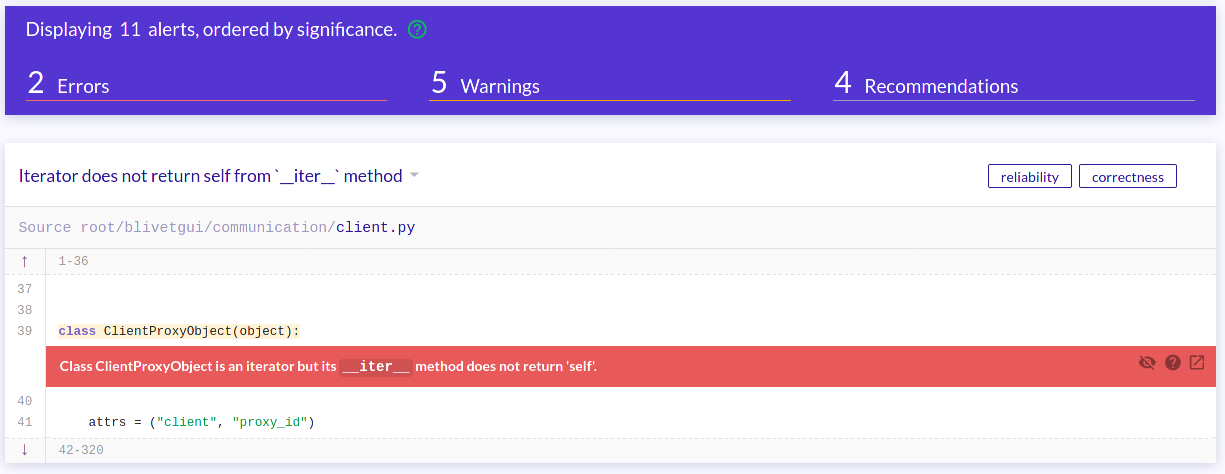
\includegraphics[width=\textwidth]{img/lgtm.png}
	\end{center}
\end{figure}

\small\url{https://lgtm.com/projects/g/storaged-project/blivet-gui/}

\end{frame}

\section{Code Style}

\begin{frame}
	\frametitle{Code style and style guides}

	\begin{block}{}
		\begin{itemize}
			\item Coding conventions -- naming, code lay-out, comment style…
			\item Language specific (PEP 8\footnotemark), project specific (Linux kernel coding style\footnotemark) or library/toolkit specific (GTK coding style\footnotemark).
			\item Automatic checks using specific tools (\texttt{pycodestyle}) or (partially) by the static analysis tools.
		\end{itemize}
	\end{block}

\footnotetext[5]{\tiny\url{https://www.python.org/dev/peps/pep-0008/}}
\footnotetext[6]{\tiny\url{https://www.kernel.org/doc/html/v5.11/process/coding-style.html}}
\footnotetext[7]{\tiny\url{https://developer.gnome.org/programming-guidelines/stable/c-coding-style.html.en}}
\end{frame}

\begin{frame}
	\frametitle{Linux kernel coding style}

\begin{center}
	\color{blue}{\url{https://www.kernel.org/doc/html/v5.11/process/coding-style.html}}
	
	\begin{figure}[ht!]
	\begin{center}
  	  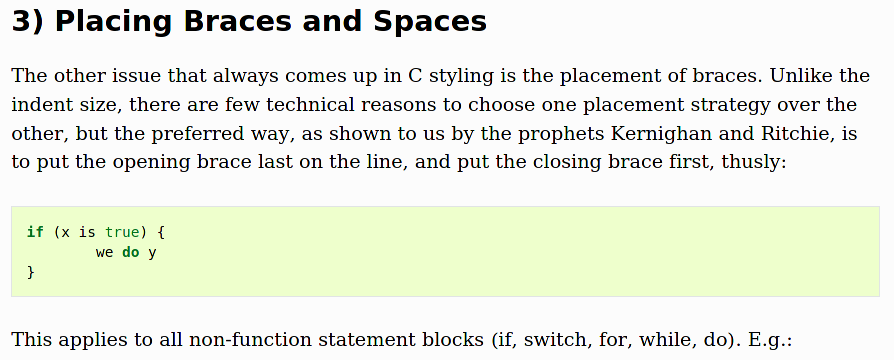
\includegraphics[width=11cm]{img/kernel-coding-styles-1.png}
	\end{center}
	\end{figure}
\end{center}
\end{frame}

\begin{frame}
	\frametitle{Python and PEP 8}

	\begin{itemize}
		\item Automatic code style checking tools exist for the Python PEP 8 style code.
		\item \texttt{pycodestyle}\footnotemark (formerly \texttt{pep8}) is used for checking/enforcing PEP 8 in many Python applications.
		\item \texttt{black}\footnotemark can be used to automatically format Python code in a PEP 8 compliant way.
		\item Static analysis tools like \texttt{pylint} or \texttt{pyflakes} also check for some PEP 8 style violations.
	\end{itemize}

\footnotetext[8]{\tiny\url{https://github.com/PyCQA/pycodestyle}}
\footnotetext[9]{\tiny\url{https://github.com/psf/black}}
\end{frame}

\begin{frame}[fragile]
	\frametitle{Python and PEP 8}

\begin{lstlisting}[frame=none, basicstyle=\ttfamily\small, columns=fullflexible, keepspaces=true]
$ pycodestyle-3 blivetgui/blivetgui.py 
blivetgui/blivetgui.py:23:80: E501 line too long (80 > 79 characters)
blivetgui/blivetgui.py:30:1: E402 module level import not at top of file
\end{lstlisting}

	\begin{figure}[ht!]
	\begin{center}
  	  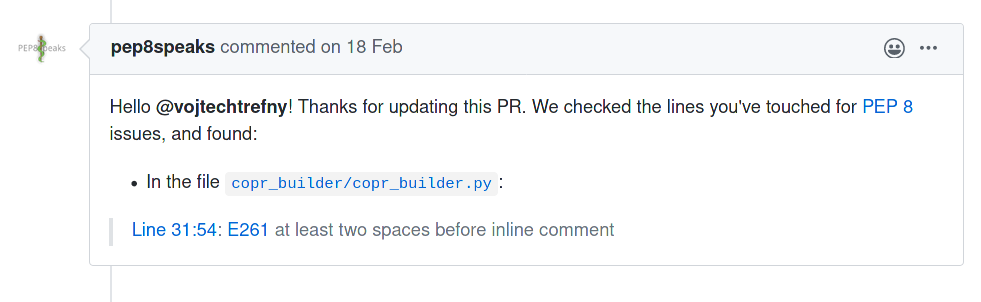
\includegraphics[width=13cm]{img/pep8speaks.png}
	\end{center}
	\end{figure}
\end{frame}

\begin{frame}
	\frametitle{Documentation style}
	
	\begin{block}{}
		\begin{itemize}
			\item Documentation might be checked in the same way code is.
			\item Similar style documents and tools for checking documentations exist (for example PEP 257\footnotemark and pydocstyle\footnotemark for Python).
			\item In some cases wrong or missing documentation (docstrings in the code) can lead to a broken build or missing features.
		\end{itemize}
	\end{block}

\footnotetext[10]{\tiny\url{https://www.python.org/dev/peps/pep-0257/}}
\footnotetext[11]{\tiny\url{http://www.pydocstyle.org}}
\end{frame}

\section{Build}

\begin{frame}
	\frametitle{Build}
	
	\begin{block}{}
		\begin{itemize}
			\item Building the project, a preparation to run the test suite.
			\item Depends on language -- mostly no-op for interpreted languages, more complicated for compiled ones.
			\item Build in the CI environment can detect issues with dependencies.
			\item Builds on different architectures can help detect issues related to endianness or data types sizes.
		\end{itemize}
	\end{block}
\end{frame}

\section{Tests}

\begin{frame}
	\frametitle{Tests}
	
	\begin{block}{}
		\begin{itemize}
			\item Running tests that are part of the project.
			\item  New tests should be part of every change to the codebase.
			\begin{itemize}
				\item New features require new unit and integration tests.
				\item Bug fixes should come with a regression test.
			\end{itemize}
			\item For some project (like libraries) running test suites of their users might be an option.
		\end{itemize}
	\end{block}
\end{frame}

\begin{frame}
	\frametitle{Coverage}
	
	\begin{block}{}
		\begin{itemize}
			\item Code coverage (or Test coverage) represents how much of the code is covered by the test suite.
			\item Usually percentual value that shows how many lines of the code were “visited” by the test.
			\item Generally a check that all functions and branches are covered by the suite.
			\item Used as a measure of the test suite “quality”.
		\end{itemize}
	\end{block}
\end{frame}

\begin{frame}[fragile]
	\frametitle{Coverage}
	
	\begin{figure}[ht!]
	\begin{center}
  	  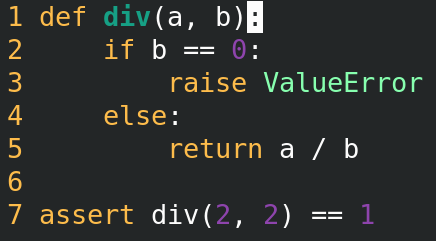
\includegraphics[width=5cm]{img/coverage-test.png}
	\end{center}
	\end{figure}
	
\begin{center}
\begin{lstlisting}[frame=none, basicstyle=\ttfamily\small, columns=fullflexible, keepspaces=true]
$ coverage3 report -m
Name      Stmts   Miss  Cover   Missing
---------------------------------------
div.py    5       1     80%     3
\end{lstlisting}
	
\color{red}{Resulting coverage is 80 \% because 1 of 5 statements is not covered.}
\end{center}
\end{frame}

\begin{frame}
	\frametitle{Coverage}
	
	\begin{block}{}
		\begin{itemize}
			\item Automated coverage tests might be part of the CI.
			\item Decrease in coverage can be viewed as a reason to reject contribution to the project.
		\end{itemize}
	\end{block}
	
	\begin{figure}[ht!]
	\begin{center}
  	  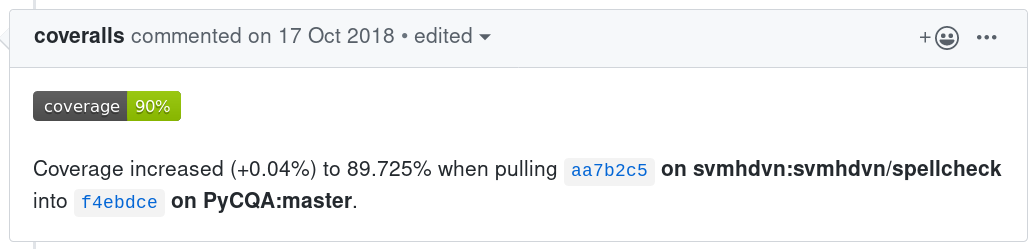
\includegraphics[width=12.5cm]{img/coverage-bot.png}
	\end{center}
	\end{figure}
\end{frame}

\section{Delivery and Deployment}

\begin{frame}
	\frametitle{Packaging and publishing}
	
	\begin{block}{}
		\begin{itemize}
			\item \textbf{Delivery} -- releasing new changes quickly and regularly (daily, weekly...).
			\item \textbf{Deployment} -- delivery with automated push to production, without human interaction.
		\end{itemize}
	\end{block}
	
	\begin{block}{}
		\begin{itemize}
			\item Usually after merging the changes, not for the PRs.
			\item Building packages, container images, ISO images…
			\item Built packages can be used for further testing (manually by the Quality Assurance or in another CI infrastructure) or directly pushed to production or included in testing/nightly builds of the project.
		\end{itemize}
	\end{block}
\end{frame}

%%%%%%%%%%%%%%%%%%%%%%%%%%%%%%%%%%%%%%%%%%%%%%%%%%%%%%%%%%%%%%%%%%

\section{CI Tools \\ \small Demo}

\begin{frame}
	\frametitle{Travis CI}
	
	\begin{columns}
\begin{column}{0.6\textwidth}
	\begin{block}{}
		\begin{itemize}
			\item Probably (still) the most popular CI service nowadays.
			\item Can be integrated into your projects on GitHub.
			\item Free (with limits) for opensource projects.
			\item Configured using \texttt{.travis.yml} file in the project
			\item Travis drastically limited free plans for opensource projects in 2020\footnotemark.
			\item \color{blue}{\url{https://travis-ci.org}}
		\end{itemize}
	\end{block}
\end{column}
\begin{column}{0.4\textwidth}
	\begin{figure}[ht!]
	\begin{center}
  	  
\includegraphics[width=0.5\textwidth]{img/travis-logo.png}
	\end{center}
	\end{figure}
\end{column}
\end{columns}

\footnotetext[12]{\tiny\url{https://blog.travis-ci.com/2020-11-02-travis-ci-new-billing}}
\end{frame}

\begin{frame}
	\frametitle{Travis CI}
	\begin{figure}[ht!]
	\begin{center}
  	  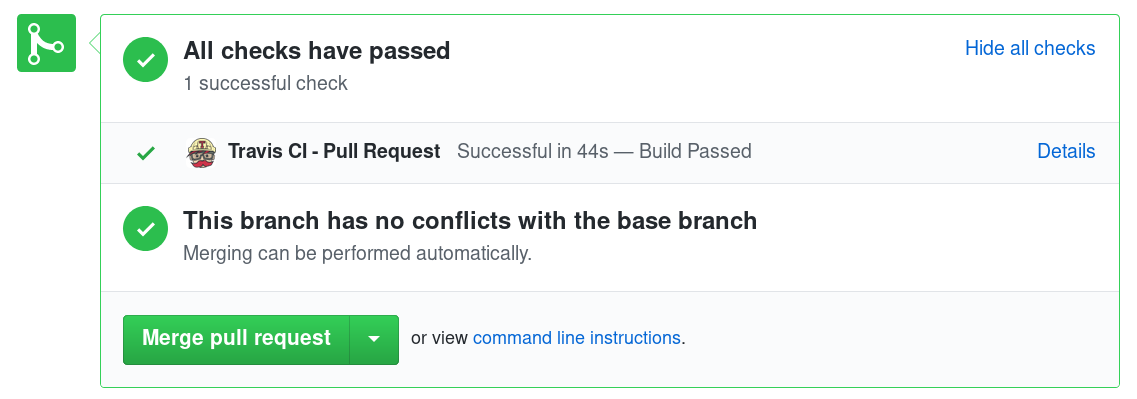
\includegraphics[width=0.9\textwidth]{img/travis-1.png}
	\end{center}
	\end{figure}
\end{frame}

\begin{frame}
	\frametitle{Travis CI}
	\begin{figure}[ht!]
	\begin{center}
  	  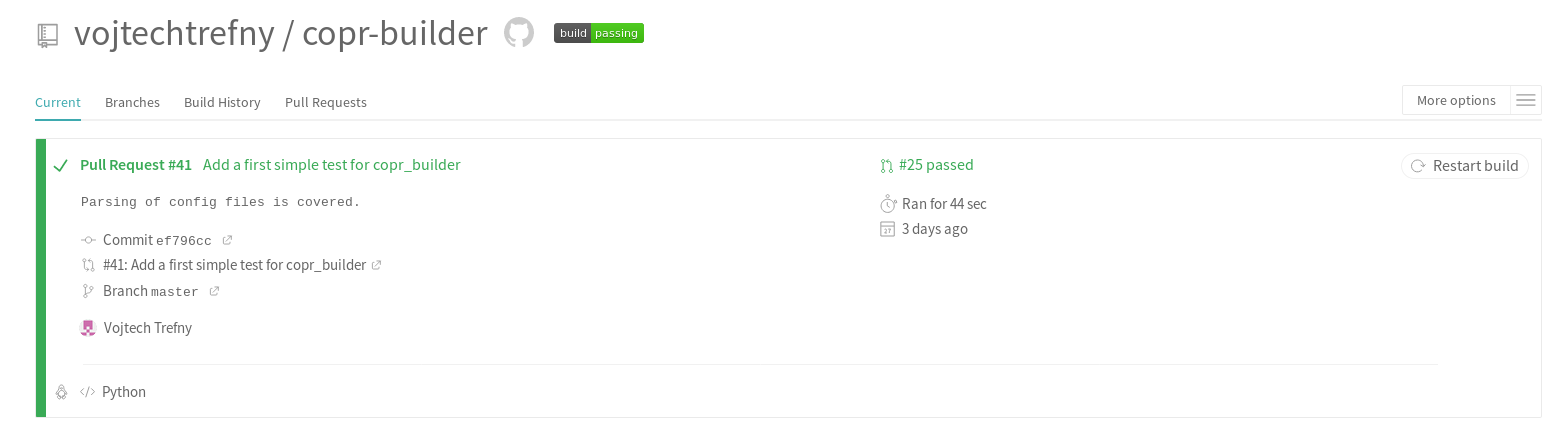
\includegraphics[width=0.9\textwidth]{img/travis-3.png}
	\end{center}
	\end{figure}
\end{frame}

\begin{frame}
	\frametitle{GitHub Actions}
	
	\begin{columns}
\begin{column}{0.6\textwidth}
	\begin{block}{}
		\begin{itemize}
			\item Automation \emph{framework} integrated into GitHub.
			\item Does not cover only CI but also CD (publishing packages on various services and deploying on many public clouds) and project and issue management.
			\item Free for all public repositories, limited and paid options for private projects.
			\item \color{blue}{\url{https://github.com/features/actions}}
		\end{itemize}
	\end{block}
\end{column}
\begin{column}{0.4\textwidth}
	\begin{figure}[ht!]
	\begin{center}
  	  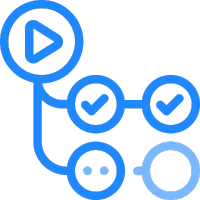
\includegraphics[width=0.5\textwidth]{img/gh-actions-logo.png}
	\end{center}
	\end{figure}
\end{column}
\end{columns}

\end{frame}

\begin{frame}
	\frametitle{GitHub Actions}
	\begin{figure}[ht!]
	\begin{center}
  	  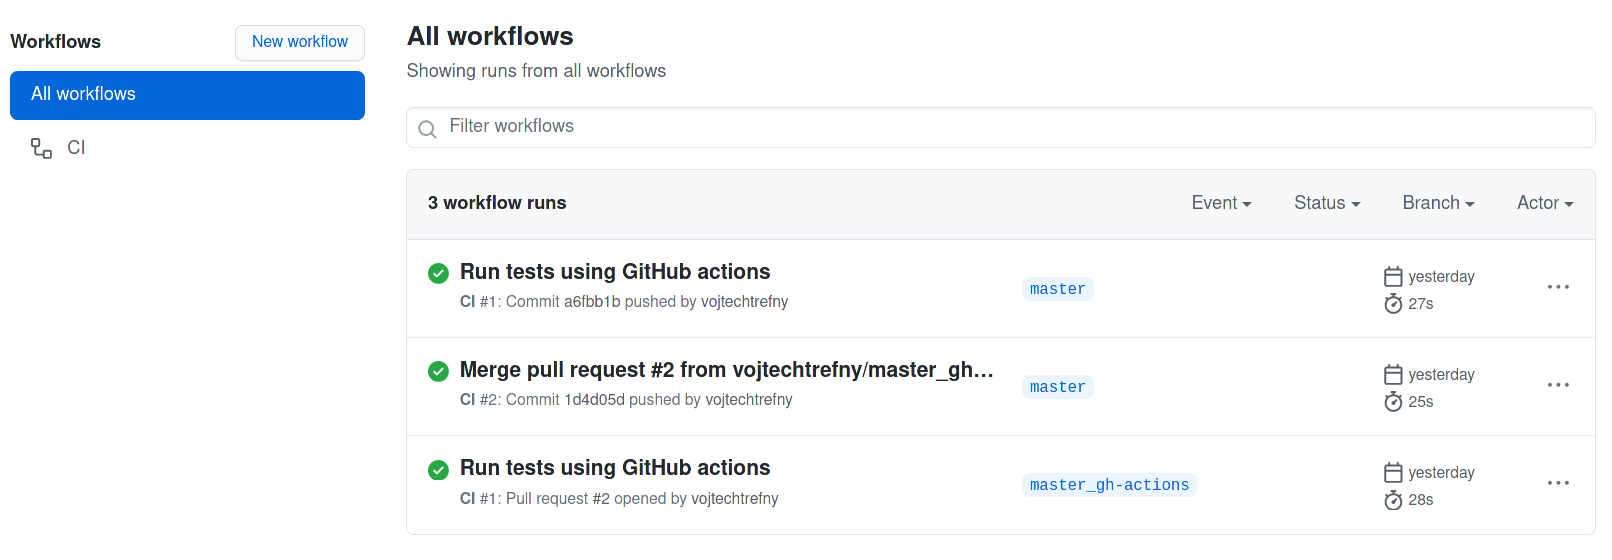
\includegraphics[width=0.9\textwidth]{img/gh-actions-1.png}
	\end{center}
	\end{figure}
\end{frame}

\begin{frame}
	\frametitle{GitHub Actions}
	\begin{figure}[ht!]
	\begin{center}
  	  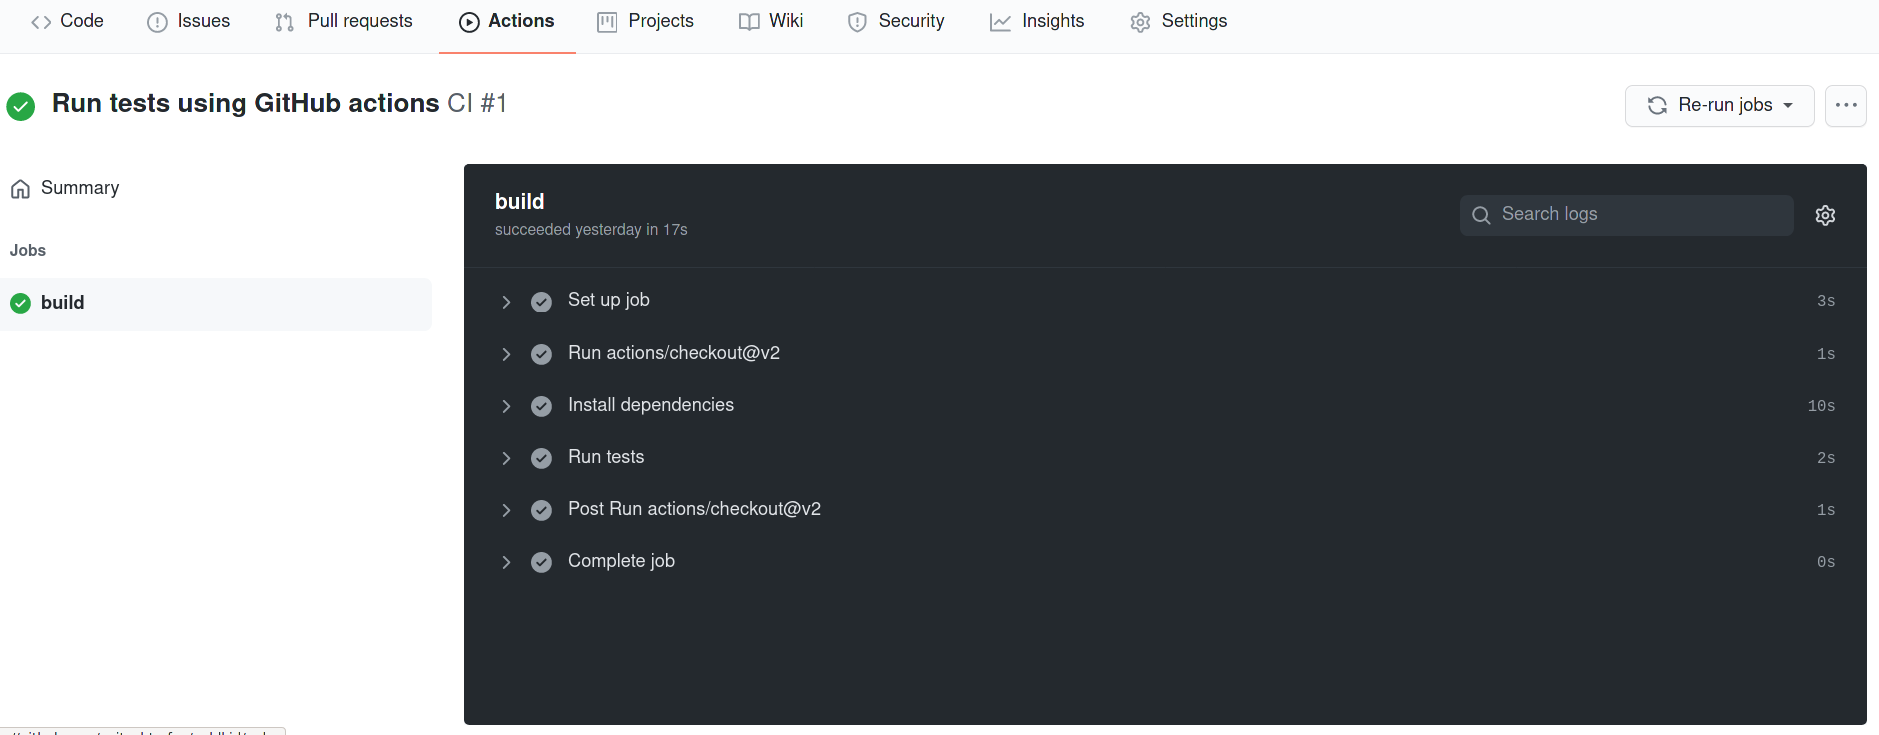
\includegraphics[width=0.9\textwidth]{img/gh-actions-2.png}
	\end{center}
	\end{figure}
\end{frame}

\begin{frame}
	\frametitle{Jenkins}
	
	\begin{columns}
\begin{column}{0.6\textwidth}
	\begin{block}{}
		\begin{itemize}
			\item Automation system, not a “true” CI/CD tool.
			\item Can automatically run given tasks on a node or set of nodes.
			\item Tasks can be started on time basis or triggered by an external event (like a new commit or PR on GitHub).
			\item \color{blue}{\url{https://jenkins.io/}}

		\end{itemize}
	\end{block}
\end{column}
\begin{column}{0.4\textwidth}
	\begin{figure}[ht!]
	\begin{center}
  	  
\includegraphics[width=0.5\textwidth]{img/jenkins.png}
	\end{center}
	\end{figure}
\end{column}
\end{columns}
\end{frame}

\begin{frame}
	\frametitle{Fedora CI}
	
	\begin{columns}
\begin{column}{0.6\textwidth}
	\begin{block}{}
		\begin{itemize}
			\item Complex CI system with the task to deliver an ``Always Ready Operating System''.
			\item Packages are tested after every change and \emph{gated} if the CI pipeline fails.
			\item The goal is to prevent breaking the distribution. CI will stop the broken package before it can affect the distribution.
		\end{itemize}
	\end{block}
\end{column}
\begin{column}{0.4\textwidth}
	\begin{figure}[ht!]
	\begin{center}
  	  
\includegraphics[width=0.5\textwidth]{img/fedora.png}
	\end{center}
	\end{figure}
\end{column}
\end{columns}
\end{frame}

\begin{frame}
	\frametitle{Fedora CI}
	\begin{figure}[ht!]
	\begin{center}
  	  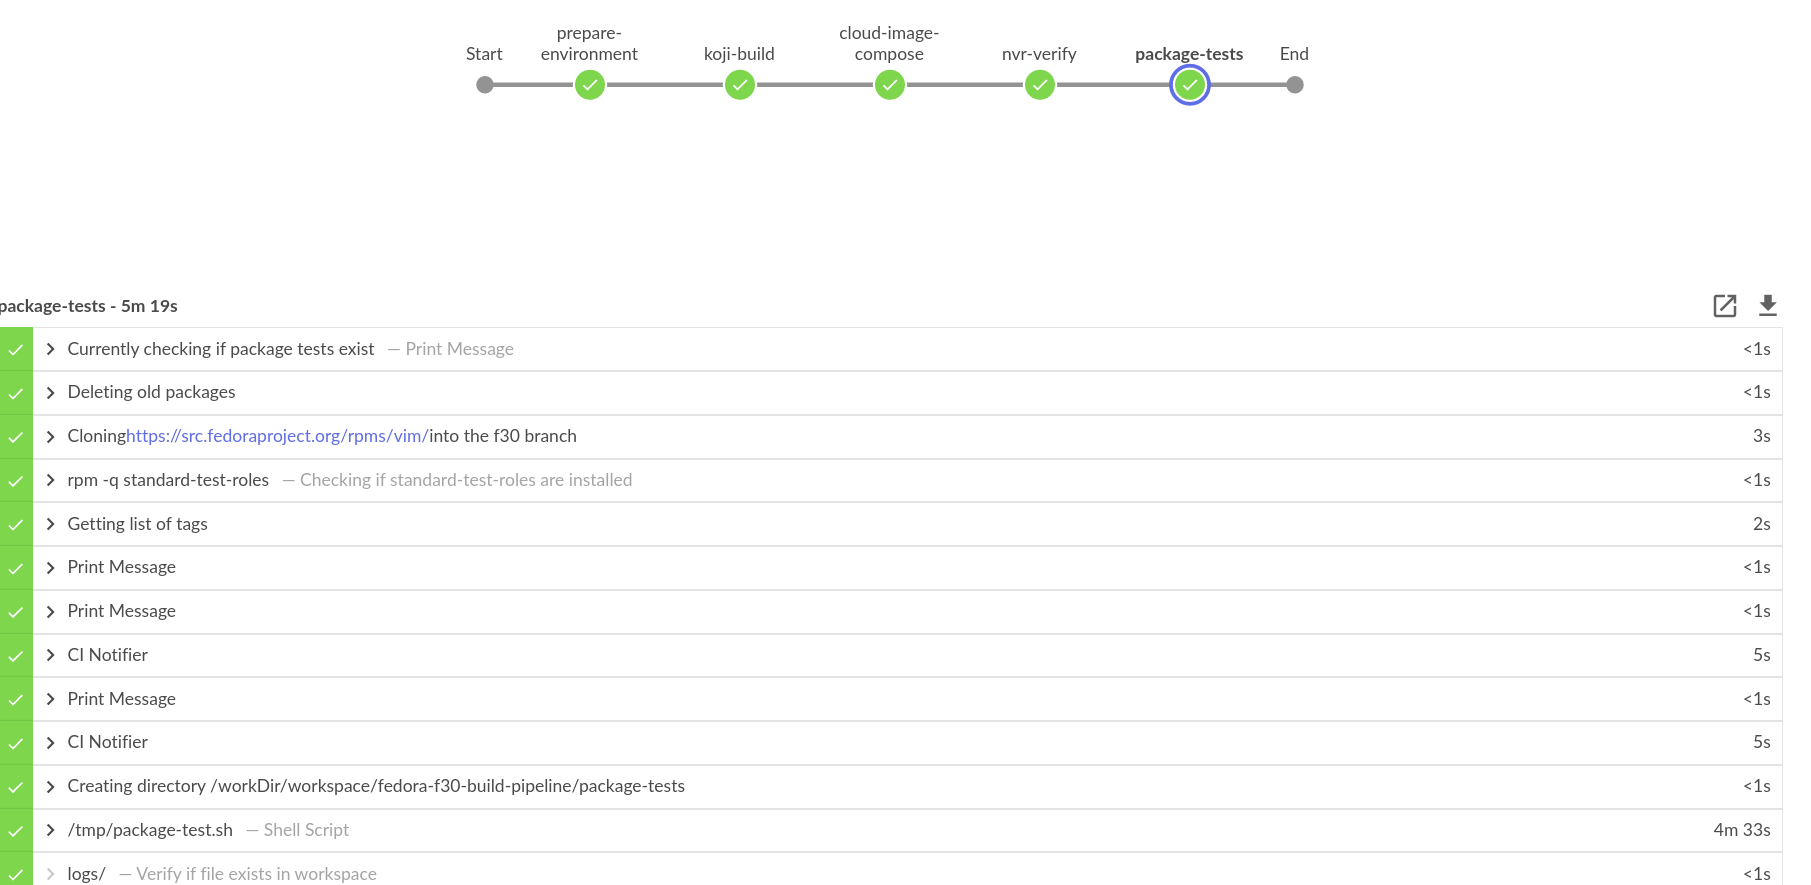
\includegraphics[width=0.9\textwidth]{img/fedora-ci-1.png}
	\end{center}
	\end{figure}
\end{frame}

\begin{frame}
	\frametitle{Packit}
	
	\begin{columns}
\begin{column}{0.6\textwidth}
	\begin{block}{}
		\begin{itemize}
			\item Tool for integrating upstream projects to Fedora.
			\item RPM packages are automatically built on every pull request.
			\item New releases can be automatically built and pushed to Fedora.
		\end{itemize}
	\end{block}
\end{column}
\begin{column}{0.4\textwidth}
	\begin{figure}[ht!]
	\begin{center}
  	  
\includegraphics[width=0.7\textwidth]{img/packit-logo.png}
	\end{center}
	\end{figure}
\end{column}
\end{columns}
\end{frame}

\begin{frame}
	\frametitle{Packit}
	\begin{figure}[ht!]
	\begin{center}
  	  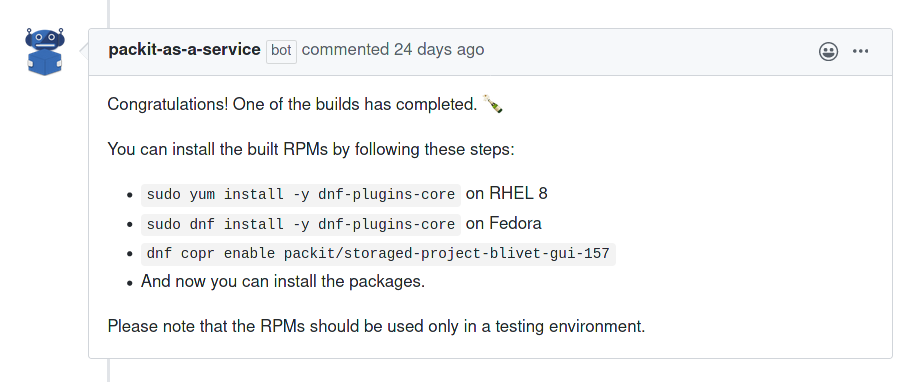
\includegraphics[width=0.9\textwidth]{img/packit-1.png}
	\end{center}
	\end{figure}
\end{frame}

%%%%%%%%%%%%%%%%%%%%%%%%%%%%%%%%%%%%%%%%%%%%%%%%%%%%%%%%%%%%%%%%%%

\section{Questions}

\begin{frame}
	\frametitle{Questions}

	\begin{center}
	Thank you for your attention.
	\end{center}

\vspace{0.5cm}

	\begin{center}
	\color{blue}{\url{https://github.com/crocs-muni/open-source-development-course}}
	\end{center}
\end{frame}

\end{document}

